\documentclass[11pt]{article}

\usepackage[margin=1.6cm]{geometry}
\usepackage{amsmath}
\usepackage{amssymb}
\usepackage{enumitem}
\usepackage{titlesec}
\usepackage{xcolor}
\usepackage{fancyhdr}
\usepackage{multicol}
\usepackage{array}
\usepackage{tikz}

\titleformat{\section}{\large\bfseries\color{blue!50!black}}{\thesection}{0.6em}{}
\titlespacing{\section}{0pt}{1.0em}{0.3em}

\setlength{\headheight}{14pt}

\pagestyle{fancy}
\fancyhf{}
\fancyhead[L]{Fractions, Probability and Trees}
\fancyfoot[C]{\thepage}
\renewcommand{\headrulewidth}{0.4pt}

\fancypagestyle{firstpage}{%
  \fancyhf{}
  \fancyhead[L]{Fractions, Probability and Trees}
  \fancyhead[R]{Name: \makebox[4cm]{\hrulefill}}
  \fancyfoot[C]{\thepage}
  \renewcommand{\headrulewidth}{0.4pt}
}

\newcommand{\ans}{\hrulefill}
\newcommand{\anshere}{\par\vspace{0.3em}\noindent\ans\par\vspace{0.3em}}
\setlist[enumerate,1]{leftmargin=1.4em, itemsep=0.3em, topsep=0.2em}
\setlength{\columnsep}{1.1cm}
\setlength{\columnseprule}{0.4pt}
\raggedcolumns

\newcolumntype{Y}{>{\centering\arraybackslash}p{1.9cm}}

\begin{document}
\thispagestyle{firstpage}

\begin{center}
  {\Large\bfseries Fractions, Probability and Trees}
\end{center}
\vspace{0.2em}

\begingroup\small

\section*{Fractions, Decimals and Percentages}
\noindent Fraction $\to$ decimal: divide. \quad Decimal $\to$ percentage: $\times 100$. \quad
Percentage $\to$ fraction: write over $100$, simplify.

\vspace{0.2em}
\begin{center}
\begin{tabular}{|Y|Y|Y|}
\hline
\textbf{Fraction} & \textbf{Decimal} & \textbf{Percentage} \\\hline
$\dfrac{1}{4}$ & & \\[0.5em]\hline
$\dfrac{3}{5}$ & & \\[0.5em]\hline
 & $0.15$ & \\[0.5em]\hline
 & & $35\%$ \\[0.5em]\hline
$\dfrac{17}{20}$ & & \\[0.5em]\hline
 & $0.08$ & \\[0.5em]\hline
$\dfrac{1}{2}$ & & \\[0.5em]\hline
$\dfrac{9}{10}$ & & \\[0.5em]\hline
 & & $20\%$ \\[0.5em]\hline
$\dfrac{3}{4}$ & & \\[0.5em]\hline
\end{tabular}
\end{center}

\vspace{0.4em}
\section*{Probability as a Decimal}
\noindent Find each probability, giving your answer as a \textbf{decimal}.

\begin{multicols}{2}
\begin{enumerate}[label=(\alph*)]
  \item A spinner has $5$ equal sections, $1$ of which is red. Find $P(\text{red})$.
  \anshere
  \item A bag has $20$ balls, $5$ of which are yellow. Find $P(\text{yellow})$.
  \anshere
  \item A class of $20$ students has $8$ who walk to school. Find $P(\text{walks})$.
  \anshere
  \item Toss a coin. Find $P(\text{heads})$.
  \anshere
  \item A spinner has $4$ equal sections, $3$ of which are green. Find $P(\text{green})$.
  \anshere
  \item A box of $50$ raffle tickets has $45$ losing tickets. Find $P(\text{losing ticket})$.
  \anshere
  \item A box of $10$ chocolates has $1$ with a caramel filling. Find $P(\text{caramel})$.
  \anshere
  \item A spinner has $20$ equal sections, $6$ of which are purple. Find $P(\text{purple})$.
  \anshere
  \item A class of $30$ students has $18$ who bring lunch from home. Find $P(\text{home
    lunch})$.
  \anshere
  \item A bag has $10$ marbles, $7$ of which are orange. Find $P(\text{orange})$.
  \anshere
  \item A spinner has $5$ equal sections, $4$ of which are gold. Find $P(\text{gold})$.
  \anshere
  \item A raffle has $20$ tickets, $1$ of which is a winning ticket. Find $P(\text{winning
    ticket})$.
  \anshere
\end{enumerate}
\end{multicols}
\endgroup

\newpage

\section*{Multistep Events: Listing Sample Spaces}
\noindent A \textbf{tree diagram} can help you list every possible outcome of a multistep
experiment --- the \textbf{sample space}. Each complete path through the tree, from start to
end, is one outcome. When every branch is equally likely, you don't need to label branches with
probabilities --- just list the outcomes systematically.

\vspace{0.3em}
\noindent\textbf{Worked example:} Flip a coin, then roll a die. List the sample space.

\begin{center}
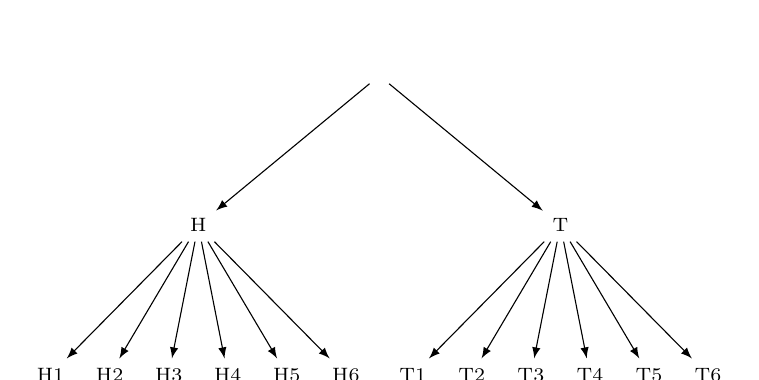
\begin{tikzpicture}[
  level distance=1.9cm,
  level 1/.style={sibling distance=4.6cm},
  level 2/.style={sibling distance=0.75cm},
  edge from parent/.style={draw, -latex},
  every node/.style={font=\scriptsize}
]
\node {}
  child { node {H}
    child { node {H1} }
    child { node {H2} }
    child { node {H3} }
    child { node {H4} }
    child { node {H5} }
    child { node {H6} }
  }
  child { node {T}
    child { node {T1} }
    child { node {T2} }
    child { node {T3} }
    child { node {T4} }
    child { node {T5} }
    child { node {T6} }
  };
\end{tikzpicture}
\end{center}
\noindent $\Omega = \{H1, H2, H3, H4, H5, H6, T1, T2, T3, T4, T5, T6\}$. There are $12$ equally
likely outcomes in total.

\vspace{0.5em}
\begin{multicols}{2}
\noindent\textbf{(a)} A spinner has three equal sections: A, B, C. After spinning, you also
toss a coin. Complete the tree diagram, then list the sample space.

\begin{center}
\begin{tikzpicture}[
  level distance=2.0cm,
  level 1/.style={sibling distance=2.7cm},
  level 2/.style={sibling distance=1.1cm},
  edge from parent/.style={draw, -latex},
  every node/.style={font=\scriptsize}
]
\node {}
  child { node {\hrulefill}
    child { node {\hrulefill} }
    child { node {\hrulefill} }
  }
  child { node {\hrulefill}
    child { node {\hrulefill} }
    child { node {\hrulefill} }
  }
  child { node {\hrulefill}
    child { node {\hrulefill} }
    child { node {\hrulefill} }
  };
\end{tikzpicture}
\end{center}
\anshere

\columnbreak

\noindent\textbf{(b)} A T-shirt comes in colour Red or Blue, and size S, M or L. Complete the
tree diagram, then list the sample space.

\begin{center}
\begin{tikzpicture}[
  level distance=2.0cm,
  level 1/.style={sibling distance=3.6cm},
  level 2/.style={sibling distance=0.95cm},
  edge from parent/.style={draw, -latex},
  every node/.style={font=\scriptsize}
]
\node {}
  child { node {\hrulefill}
    child { node {\hrulefill} }
    child { node {\hrulefill} }
    child { node {\hrulefill} }
  }
  child { node {\hrulefill}
    child { node {\hrulefill} }
    child { node {\hrulefill} }
    child { node {\hrulefill} }
  };
\end{tikzpicture}
\end{center}
\anshere
\end{multicols}

\vspace{0.3em}
\begin{enumerate}[label=(\alph*)]
\setcounter{enumi}{2}
  \item A meal deal lets you choose one starter (Soup or Salad) and one main (Pasta, Pizza or
    Fish). List all possible meal combinations.
  \anshere
  \item \textbf{Extension:} A coin is tossed three times. List all possible outcomes. (Hint:
    there are $8$.)
  \anshere
\end{enumerate}

\end{document}
